\part{Sharing the Medium}

\chapter{Random Access: From ALOHA to Framed Slots}
\label{ch:aloha}

\begin{defbox}[In this chapter you will learn]
\begin{itemize}
 \item why devices that cannot listen before they talk need \emph{random access};
 \item how to derive the throughput of pure and slotted ALOHA from the Poisson model;
 \item \emph{framed} slotted ALOHA, the scheme used by RFID readers and by Amber's registration and custom protocols: expected idle, success and collision slots, and the optimal frame size;
 \item how a reader can estimate the number of contenders and adapt its frame (Schoute, EPC Gen2's $Q$-algorithm), and how Amber's custom demo does it;
 \item why an \emph{energy-limited} network wants different parameters from a throughput-limited one, and how subcarrier shifts multiply capacity.
\end{itemize}
\end{defbox}

\section{The problem: many talkers, one channel}
\label{sec:aproblem}

A base station illuminates, say, a hundred nodes. When it asks ``who is there?'',
every node would like to answer at once; all answers share the same carrier. If two
reflections overlap in time on the same frequency they interfere, and (unless capture or
interference cancellation rescues them; Chapter~\ref{ch:sic}) neither is decoded.

The classical remedies are \emph{scheduling} (the base station assigns each node a
slot) and \emph{random access} (each node picks a slot by itself). Scheduling needs the
base station to know who exists; discovering who exists is precisely the problem. Hence
random access. For a battery-free node there is a second reason: \emph{it cannot
sense the channel}. Carrier-sense multiple access (CSMA), the workhorse of Wi-Fi, requires
a receiver that is awake and sensitive before every transmission---far beyond a
microwatt budget. So the only practical rule is \emph{``transmit once, at a random time
the reader has authorised''}.

\section{Pure ALOHA}
\label{sec:pure}

Norman Abramson's ALOHA system \citep{abramson1970} let radio terminals in Hawaii
transmit whenever they liked. Model it as follows. Packets have duration $T$. New
transmission attempts form a Poisson process with an average of $g$ attempts per
packet time (the \emph{offered load}). A packet starting at time $t_0$ is successful
if no other packet starts in the \emph{vulnerable interval} $(t_0-T,\,t_0+T)$, which has
length $2T$. For a Poisson process the probability of no arrival in an
interval of length $2T$ is $\e^{-2g}$. Throughput (successes per packet time) is
\begin{equation}
 s_{\mathrm{pure}}(g)=g\,\e^{-2g},\qquad s_{\max}=\frac{1}{2\e}\approx0.184\ \text{at}\ g=\tfrac12.
\end{equation}

\section{Slotted ALOHA}
\label{sec:slotted}

If time is divided into slots of length $T$ and everyone must start at a slot boundary, two packets collide
only if they choose the \emph{same} slot. The vulnerable interval shrinks to
$T$, and
\begin{equation}
 s_{\mathrm{slot}}(g)=g\,\e^{-g},\qquad s_{\max}=\frac1{\e}\approx0.368\ \text{at}\ g=1.
\label{eq:slotted}
\end{equation}
Synchronisation doubles the efficiency \citep{roberts1975}.

\begin{figure}[t]
\centering
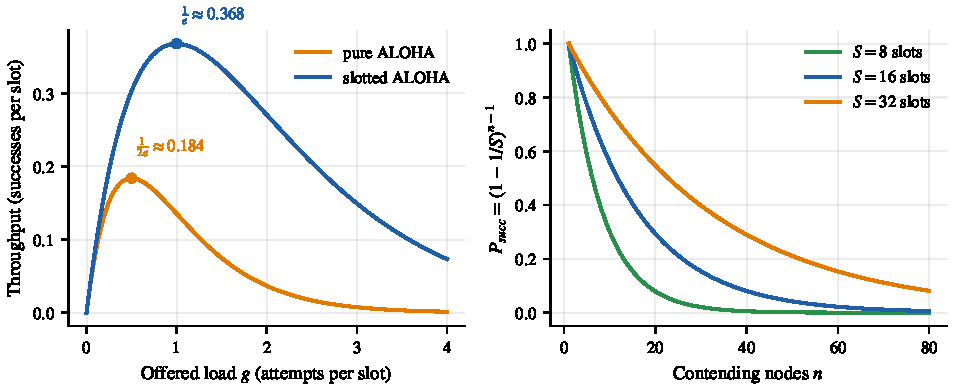
\includegraphics[width=0.95\linewidth]{fig_aloha}
\caption{Left: throughput of pure and slotted ALOHA. Right: the success probability of a single node in a frame of $S$ slots when $n$ nodes contend (Eq.~\eqref{eq:psucc}).}
\label{fig:aloha}
\end{figure}

\begin{intuition}[Why does the curve fall for large $g$?]
Throughput $=$ load $\times$ probability of success. Raising the load first
helps (more attempts) and then hurts (each attempt is more likely to collide). The maximum balances the two at $g=1$: on average exactly one attempt per slot.
\end{intuition}

\section{Framed slotted ALOHA}
\label{sec:fsa}

RFID readers, and Amber's registration, use \emph{framed} slotted ALOHA (FSA). The
base station announces a \emph{frame} of $S$ slots; each of the $n$ contending
nodes picks one slot uniformly at random and answers there. Because the number of
nodes is finite and they choose independently, the analysis is a balls-into-bins problem.

\paragraph{Slot statistics.}
The number of nodes in a given slot is Binomial$(n,1/S)$. Hence
\begin{align}
 \Pr[\text{slot idle}]&=\Big(1-\tfrac1S\Big)^{n},\\
 \Pr[\text{slot has exactly one node}]&=\frac nS\Big(1-\tfrac1S\Big)^{n-1},\\
 \Pr[\text{collision}]&=1-\text{(the two above)}.
\end{align}
The expected numbers of idle, successful and collision slots in a frame are
\begin{equation}
 E_0=S\Big(1-\tfrac1S\Big)^{n},\qquad E_1=n\Big(1-\tfrac1S\Big)^{n-1},\qquad E_c=S-E_0-E_1,
\label{eq:fsaexp}
\end{equation}
and a single node succeeds with probability
\begin{equation}
 P_{\mathrm{succ}}=\Big(1-\tfrac1S\Big)^{n-1}\;\approx\;\e^{-n/S}
\label{eq:psucc}
\end{equation}
(nobody else chose its slot). The \emph{slot efficiency} is
\begin{equation}
 \eta_S=\frac{E_1}{S}=\frac nS\Big(1-\tfrac1S\Big)^{n-1}\;\xrightarrow{S\to\infty}\;\frac nS\,\e^{-n/S}.
\end{equation}
Maximising over $S$ gives the \textbf{optimal frame size $S=n$}, with efficiency
$\approx1/\e=0.368$. Figure~\ref{fig:frameeff} shows the curves.

\begin{figure}[t]
\centering
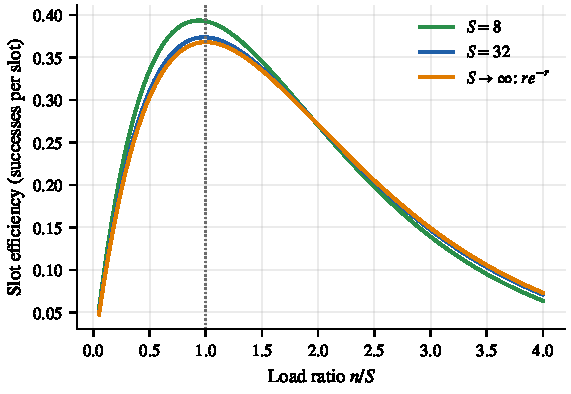
\includegraphics[width=0.58\linewidth]{fig_frame_efficiency}
\caption{Slot efficiency of framed slotted ALOHA against the load ratio $n/S$. All curves peak near $n/S=1$ at about $0.37$--$0.39$; the $S\to\infty$ limit is $re^{-r}$.}
\label{fig:frameeff}
\end{figure}

\begin{example}[A frame with 20 nodes and 16 slots]
By Eq.~\eqref{eq:fsaexp}: $E_0=16(15/16)^{20}=4.40$ idle slots; $E_1=20(15/16)^{19}=5.87$ successes; $E_c=5.73$ collision slots; efficiency $5.87/16=0.367$. Each node succeeds with probability $(15/16)^{19}=0.293$. Roughly seven of the twenty nodes are \emph{not} served in this frame, and a second frame is needed for them.
\end{example}

\paragraph{Multi-frame inventory.}
In an inventory the reader repeats frames until every node is identified. Suppose it could always
choose $S=n_k$, the number of nodes still unidentified. A frame then identifies
$E_1=n_k(1-1/n_k)^{n_k-1}\approx n_k/\e$ of them in expectation, so
\[
 n_{k+1}\approx n_k\Big(1-\tfrac1{\e}\Big)=0.63\,n_k,
\]
and the unidentified population decays geometrically. Going from $n=100$ to below one node takes
$\ln100/\ln(1/0.632)\approx10$ frames. The practical lesson is that \emph{the right frame size shrinks as nodes are identified}, so the reader has to keep estimating $n_k$.

\section{Estimating the number of contenders}
\label{sec:estimate}

The reader observes only the \emph{outcome} of each slot: idle ($c_0$ of them), success ($c_1$) or
collision ($c_c$). Schoute \citep{schoute1983} showed that at the optimal operating point a collision slot holds on average $2.39$ nodes, giving the estimate
\begin{equation}
 \hat n=c_1+2.39\,c_c.
\end{equation}
A simple lower bound is $n\ge c_1+2c_c$. EPC's Gen2 standard \citep{epcgen2} implements a variant of dynamic framing
through its \emph{$Q$-algorithm}: the frame has $2^Q$ slots and the reader adjusts a floating-point $Q_{fp}$ by
$\pm C$ after each collision (increase) or idle (decrease) slot.

\paragraph{Amber's custom protocol.}
The shipped \codew{custom_protocol} demo implements an adaptive FSA in the spirit of the
$Q$-algorithm (its docstring says ``EPC-Gen2 Q-algorithm style''). After each frame the base station
\begin{enumerate}
 \item counts $\text{heard}$ (decoded replies) and $\text{collided}$ (replies lost to collisions) and
   forms the number of contenders $m=\text{heard}+\text{collided}$ (each transmission increments exactly one of
   the two counters);
 \item smooths it, $\ell\leftarrow0.75\,\ell+0.25\,m$;
 \item sets a target frame size $\min\{32,\max\{2,\mathrm{round}(2\ell)\}\}$ and moves the actual frame size \emph{one slot} toward it, with a one-slot dead band above the target.
\end{enumerate}
Two comments. First, the base station here knows $m$ \emph{exactly}, because the simulator logs every colliding
packet individually; a real reader sees only that a slot collided (and would estimate $n$ with Schoute's formula).
This is an idealisation. Second, the target $S=2\ell$ is not the throughput-optimal $S=n$; the next section shows why that
can be a good choice here.

\section{An energy-aware twist}
\label{sec:energytwist}

In RFID a collision wastes \emph{airtime}. In an Ambient IoT node it also wastes \emph{joules}:
the node has already paid for the transmission. With the demo's numbers, a transmission
costs about $E_{\mathrm{tx}}\approx\SI{112}{\micro J}$ (Chapter~\ref{ch:controller}). The expected energy per \emph{successfully delivered} packet is
\begin{equation}
 \bar E_{\mathrm{deliv}}=\frac{E_{\mathrm{tx}}}{P_{\mathrm{succ}}}=\frac{E_{\mathrm{tx}}}{(1-1/S)^{n-1}}.
\end{equation}
\begin{center}
\small
\renewcommand{\arraystretch}{1.1}
\begin{tabular}{@{}lrrr@{}}
\toprule
$n=30$ nodes & slot efficiency & $P_{\mathrm{succ}}$ & energy per delivered packet\\
\midrule
$S=n=30$ & $0.374$ & $0.374$ & $\SI{299}{\micro J}$\\
$S=2n=60$ & $0.307$ & $0.614$ & $\SI{182}{\micro J}$\\
\bottomrule
\end{tabular}
\end{center}
Doubling the frame costs about $18\%$ of slot efficiency but cuts the energy spent per delivered packet by $39\%$.
\begin{keyidea}
A frame-size policy that is optimal for \emph{airtime} is not optimal for \emph{energy}. When every transmission
drains a scarce capacitor, a larger frame ($S>n$) is worth its idle slots. This is exactly the trade-off that Amber lets you explore, and a reason the
demo's rule-of-thumb $S\approx2\ell$ is sensible.
\end{keyidea}
There is a second coupling: the \emph{effective} $n$ is the number of nodes that are \emph{awake} when the frame is announced, which varies with their capacitors. The base station cannot observe that number (Chapter~\ref{ch:protocols}).

\section{Several orthogonal channels: subcarrier shifts}

With $K$ mutually orthogonal subcarrier shifts (Chapter~\ref{ch:backscatter}) and nodes spread evenly over them, collisions occur only among nodes with the same shift. Each group of
$n/K$ nodes runs an independent FSA in the same $S$ time slots, so the per-node success probability is $(1-1/S)^{n/K-1}$. If instead each node picked its
(slot, shift) pair uniformly at random, the number of independent resources would be $KS$ and
$P_{\mathrm{succ}}=(1-1/(KS))^{n-1}\approx\e^{-n/(KS)}$: the same to first order. Shifts and slots are
interchangeable currencies: $K$ shifts of $S$ slots give the collision behaviour of $KS$ slots at the
airtime cost of $S$. For $n=60$, $S=10$, $K=3$ the success probability is $(1-1/30)^{59}=0.135$.

\section{From the model to the simulator}

Amber reproduces the framed structure literally. The base station's schedule is a list of
RX windows, \emph{each window being one slot}; a node chooses \codew{random.randint(0, len(rx_slots)-1)}, uniformly, among the slots advertised
(Chapter~\ref{ch:bsmodule}). Three simulator details modify the textbook picture and will be analysed in Chapters~\ref{ch:sic} and~\ref{ch:bsengine}:
\begin{enumerate}
 \item the base station advertises the slots of the \emph{current and the next} frame, so only about half of the contenders
   can answer in a given frame;
 \item two nodes in the same slot collide only if they transmit within a $\SI{5}{ms}$ \emph{time window} of each other
   (they are not forced to transmit at the slot start), and only if they share a subcarrier shift;
 \item capture and SIC resolve some collisions that the classical model counts as lost.
\end{enumerate}
All three make Amber \emph{more optimistic} than Eq.~\eqref{eq:psucc} for the \emph{collision} aspect, and the first makes it \emph{slower} per frame.

\section{Chapter summary}
\begin{itemize}
 \item Battery-free nodes cannot carrier-sense, so the reader must authorise random-access slots.
 \item Pure ALOHA peaks at $1/(2e)\approx0.184$, slotted ALOHA at $1/e\approx0.368$.
 \item Framed slotted ALOHA: $E_1=n(1-1/S)^{n-1}$, $P_{\mathrm{succ}}=(1-1/S)^{n-1}\approx\e^{-n/S}$, optimum $S=n$.
 \item Schoute's estimator $\hat n=c_1+2.39\,c_c$ underlies adaptive framing; Amber's custom demo uses its own exact counts.
 \item For energy-limited tags a larger frame ($S\approx2n$) can minimise energy per delivered packet.
 \item $K$ orthogonal subcarrier shifts act like $K$ times as many slots.
\end{itemize}

\begin{codemap}
\small
\begin{tabularx}{\linewidth}{@{}>{\ttfamily}p{5.2cm}X@{}}
\toprule
\normalfont\bfseries Concept & \normalfont\bfseries Code\\
\midrule
Random slot choice & \codew{BackscatterModule.handle_command} (\codew{random.randint})\\
Frame = TX command + $S$ RX windows & schedule entries \code{("tx",...)}, \code{("rx",...)} in \file{bsengine.py}\\
Adaptive frame size & \codew{adaptive_aloha_policy} in \file{custom_protocol_demo.py}\\
Contender count & \codew{decoded_this_frame}, \codew{total_collided}\\
\bottomrule
\end{tabularx}
\end{codemap}

\section*{Exercises}
\begin{exercise}
Derive the pure-ALOHA throughput and its maximum. Why is the vulnerable period twice as long as in the slotted case?
\end{exercise}
\begin{exercise}
For $n=20$ nodes and $S=16$ slots compute $E_0$, $E_1$, $E_c$ and the efficiency (verify the worked example). How many slots would maximise efficiency, and what would it be?
\end{exercise}
\begin{exercise}
After a frame of $S=16$ slots the reader observes $c_0=6$, $c_1=5$, $c_c=5$. Estimate the number of contenders using Schoute's formula and the lower bound. Which frame size should it use next?
\end{exercise}
\begin{exercise}
Compute the energy per delivered packet for $n=30$ and $S\in\{30,45,60,90\}$ when $E_{\mathrm{tx}}=\SI{112}{\micro J}$ and compare with the slot efficiency. Where would you set the frame size if idle slots cost nothing but airtime counts against latency?
\end{exercise}
\begin{exercise}
$n=60$ nodes are divided equally among $K=3$ subcarrier shifts and all reply in a frame of $S=10$ slots. Compute the per-node success probability, and compare with $K=1$.
\end{exercise}
